\subsubsection{Q10.20 data 10312021 grouped by scenario \& x_first}

\begin{comment}
                     EFPR        EO      EFNR     n    pvalue
(frauth, False)  0.461538  0.538462  0.461538  13.0  0.630760
(frauth, True)   0.562500  0.437500  0.375000   8.0  0.563703
(icu, False)     0.600000  0.400000  0.700000   5.0  0.625000
(icu, True)      0.750000  0.250000  0.571429  14.0  0.039000
(rent, False)    0.350000  0.650000  0.350000  10.0  0.165518
(rent, True)     0.409091  0.590909  0.681818  11.0  0.962912
\end{comment}

\begin{table}[h]
    \centering
    \begin{tabular}{|c|c|c|c|c|c|c|}
        \hline
        scenario & x_first & EFPR & EO & EFNR & n & p-value\\
        \hline
        frauth & False & 0.462 & \textbf{0.538} & 0.462 & 13.0 & 0.631\\
		frauth & True & \textbf{0.562} & 0.438 & 0.375 & 8.0 & 0.564\\
		icu & False & \textbf{0.600} & 0.400 & \textbf{0.700} & 5.0 & 0.625\\
		icu & True & \textbf{0.750} & 0.250 & \textbf{0.571} & 14.0 & \textbf{0.039}\\
		rent & False & 0.350 & \textbf{0.650} & 0.350 & 10.0 & 0.166\\
		rent & True & 0.409 & \textbf{0.591} & \textbf{0.682} & 11.0 & 0.963\\
		
        \hline
    \end{tabular}
    \caption{Grouped by scenario x_first}
    \label{tab:my_label}
\end{table}
\begin{figure}[h]
    \centering
    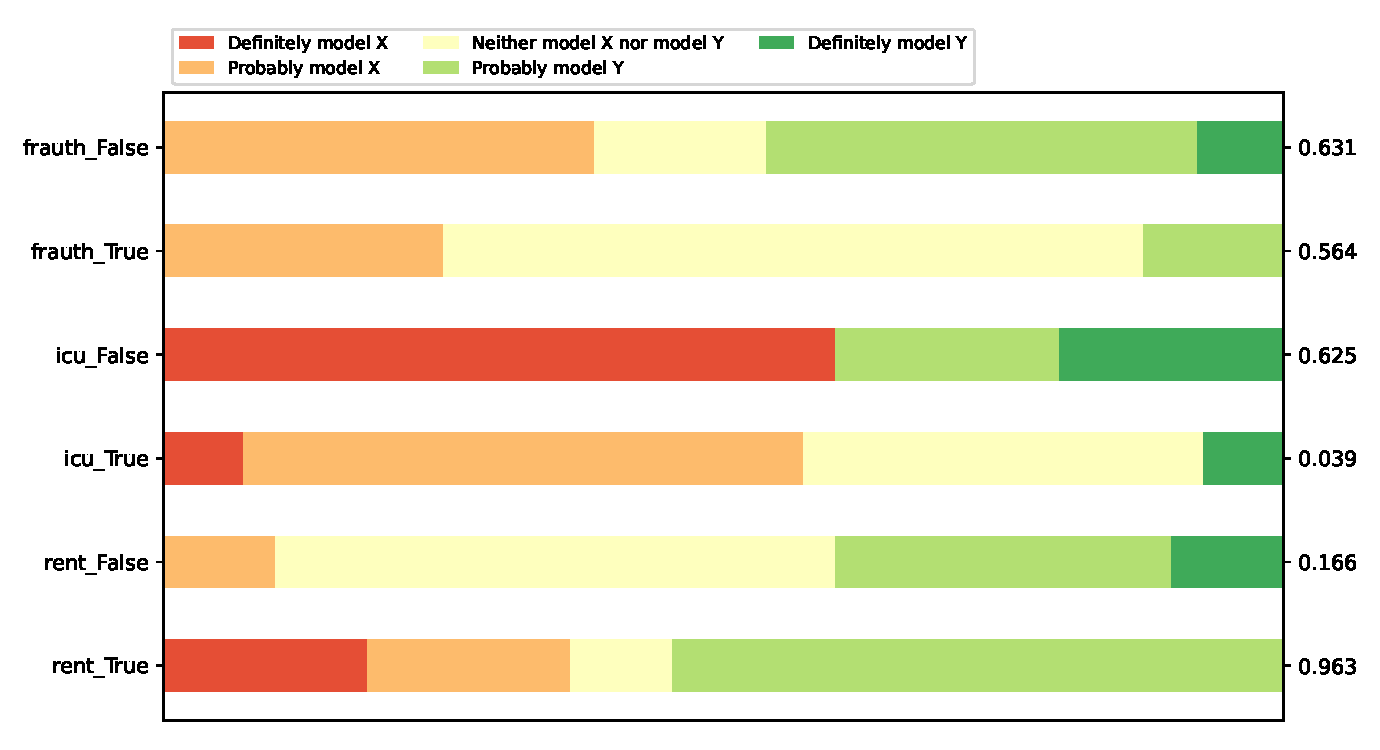
\includegraphics[width=0.8\textwidth]{figures/Q10.20/10312021/Q10.20_scenario_x_first.pdf}
    \caption{Grouped by scenario \& x_first}
    \label{fig:my_label}
\end{figure}
